\documentclass[12pt,a4paper]{article}

\usepackage{fontspec}
\setmainfont{texgyrepagella}[
    Extension=.otf,
    UprightFont=*-regular,
    BoldFont=*-bold,
    ItalicFont=*-italic,
    BoldItalicFont=*-bolditalic,
    Ligatures=TeX
]
\setsansfont{texgyrepagella}[
    Extension=.otf,
    UprightFont=*-regular,
    BoldFont=*-bold,
    ItalicFont=*-italic,
    BoldItalicFont=*-bolditalic,
    Ligatures=TeX
]
\setmonofont{texgyrecursor}[
    Extension=.otf,
    UprightFont=*-regular,
    BoldFont=*-bold,
    ItalicFont=*-italic,
    BoldItalicFont=*-bolditalic,
    Scale=0.94
]

\usepackage[a4paper,margin=2.05cm]{geometry}
\usepackage{xcolor}
\usepackage{graphicx}
\usepackage{booktabs}
\usepackage{tabularx}
\usepackage{longtable}
\usepackage{array}
\usepackage{float}
\usepackage{enumitem}
\usepackage{hyperref}
\usepackage[most]{tcolorbox}
\usepackage{listings}
\usepackage{amsmath,amssymb}
\usepackage{tikz}
\usetikzlibrary{arrows.meta,positioning,calc,shapes.geometric}

\graphicspath{{../outputs/}}
\hypersetup{colorlinks=true, linkcolor=blue, urlcolor=blue}

\definecolor{Primary}{HTML}{1F2937}
\definecolor{Accent}{HTML}{2563EB}
\definecolor{Green}{HTML}{15803D}
\definecolor{Orange}{HTML}{EA580C}
\definecolor{Red}{HTML}{DC2626}
\definecolor{Purple}{HTML}{7C3AED}
\definecolor{SoftBlue}{HTML}{EFF6FF}
\definecolor{SoftGreen}{HTML}{F0FDF4}
\definecolor{SoftOrange}{HTML}{FFF7ED}
\definecolor{SoftRed}{HTML}{FEF2F2}
\definecolor{SoftPurple}{HTML}{F5F3FF}
\definecolor{Muted}{HTML}{475569}

\newcommand{\code}[1]{\texttt{#1}}
\newcommand{\term}[1]{\textbf{#1}}

\newtcolorbox{teachbox}[1]{
    enhanced,
    breakable,
    colback=SoftBlue,
    colframe=Accent,
    title={#1},
    fonttitle=\bfseries\sffamily,
    sharp corners=all
}

\newtcolorbox{saybox}[1]{
    enhanced,
    breakable,
    colback=SoftGreen,
    colframe=Green,
    title={#1},
    fonttitle=\bfseries\sffamily,
    sharp corners=all
}

\newtcolorbox{warnbox}[1]{
    enhanced,
    breakable,
    colback=SoftOrange,
    colframe=Orange,
    title={#1},
    fonttitle=\bfseries\sffamily,
    sharp corners=all
}

\newtcolorbox{rubricbox}[1]{
    enhanced,
    breakable,
    colback=SoftPurple,
    colframe=Purple,
    title={#1},
    fonttitle=\bfseries\sffamily,
    sharp corners=all
}

\setlist[itemize]{leftmargin=1.35em,itemsep=0.25em,topsep=0.25em}
\setlist[enumerate]{leftmargin=1.55em,itemsep=0.25em,topsep=0.25em}
\lstset{
    basicstyle=\ttfamily\small,
    breaklines=true,
    frame=single,
    columns=fullflexible,
    backgroundcolor=\color{gray!6}
}

\begin{document}

\begin{titlepage}
\centering
\vspace*{1cm}
{\sffamily\bfseries\Huge Tài Liệu Giảng Bài Và Kịch Bản Thuyết Trình\par}
\vspace{0.35cm}
{\sffamily\Large Ứng dụng ANN làm heuristic cho A* trong bài toán tìm đường mê cung\par}
\vspace{1cm}
{\Large Nhóm Tờ Linh: Nguyễn Quốc Minh, Võ Nguyễn Tấn Tài\par}
\vspace{0.5cm}
{\large Dùng để luyện nói, demo, giải thích code và trả lời phản biện\par}
\vfill
{\large 2026\par}
\end{titlepage}

\tableofcontents
\newpage

\section{Mục Tiêu Của Tài Liệu}

Tài liệu này được viết theo kiểu \term{giảng lại bài}, không chỉ liệt kê ý trên slide. Khi thuyết trình, người nói cần giải thích được vì sao bài toán cần ANN, ANN học như thế nào, validation khác test ra sao, và cách ANN được đưa vào A*.

\begin{rubricbox}{Bám Sát Rubric Chấm Điểm}
\begin{tabularx}{\linewidth}{>{\bfseries}p{0.27\linewidth}X}
\toprule
Tiêu chí & Cách thể hiện trong bài nói \\
\midrule
Lý thuyết 25\% & Giảng ANN từ neuron, lớp Dense, forward propagation, loss, backpropagation, epoch. Phân biệt rõ train, validation, test bằng ví dụ trực quan. \\
Thực nghiệm 35\% & Dùng ba đồ thị \code{underfit\_loss.png}, \code{overfit\_loss.png}, \code{goodfit\_loss.png}. Chỉ ra dấu hiệu underfit, overfit, good fit trên đồ thị train thật. \\
Sáng tạo 20\% & Không chỉ train model; model ANN được tích hợp vào A* làm heuristic. Demo so sánh BFS, A* + Manhattan, A* + ANN. \\
Trung thực 20\% & Nói rõ code tự cài theo module; AI hỗ trợ khung/debug/tổ chức nội dung; nhóm tự chạy dataset, train, đọc metric và giải thích cấu hình. \\
\bottomrule
\end{tabularx}
\end{rubricbox}

\begin{teachbox}{Thông điệp chính cần nhớ}
Đề tài sinh map mê cung ngẫu nhiên, dùng BFS để tạo nhãn khoảng cách thật, huấn luyện ANN bằng Keras để dự đoán khoảng cách còn lại, rồi dùng dự đoán đó làm heuristic cho A*.

Ba câu phải nói chắc:
\begin{itemize}
    \item BFS không sinh map. Map sinh ngẫu nhiên trong \code{maze.py}.
    \item BFS dùng để tạo nhãn \code{true\_distance} cho ANN.
    \item ANN được xây bằng Keras API qua \code{tf.keras} và được đưa vào A* qua \code{AnnHeuristic}.
\end{itemize}
\end{teachbox}

\section{Cách Mở Đầu Bài Thuyết Trình}

\begin{saybox}{Kịch bản mở đầu 45--60 giây}
Em xin chào thầy/cô và các bạn. Nhóm em thực hiện đề tài ứng dụng mạng nơ-ron nhân tạo làm hàm heuristic cho thuật toán A* trong bài toán tìm đường mê cung. Bình thường A* dùng heuristic Manhattan, tức một công thức cố định dựa trên tọa độ. Nhóm em thử thay heuristic đó bằng một mô hình ANN học từ dữ liệu. Dữ liệu được sinh từ nhiều map mê cung ngẫu nhiên, còn nhãn khoảng cách thật được tính bằng BFS. Sau khi train, mô hình ANN dự đoán chi phí còn lại đến goal và giá trị đó được đưa vào A* để quyết định thứ tự duyệt node.
\end{saybox}

\section{Phần Giảng Lý Thuyết 1: Bài Toán Mê Cung Và Tìm Kiếm}

\subsection{Mê cung được biểu diễn như thế nào?}

Mê cung là một ma trận 20x20. Mỗi ô có một trong hai trạng thái:

\begin{center}
\begin{tabular}{cl}
\toprule
Giá trị & Ý nghĩa \\
\midrule
0 & Đường đi, agent có thể đứng hoặc đi qua. \\
1 & Tường/vật cản, agent không được đi qua. \\
\bottomrule
\end{tabular}
\end{center}

Agent đi 4 hướng: lên, xuống, trái, phải. Mỗi bước có chi phí bằng 1. Vì mọi cạnh đều cùng chi phí, bài toán này là đồ thị không trọng số.

\begin{teachbox}{Liên hệ mã nguồn}
\code{src/maze.py} định nghĩa \code{FREE = 0}, \code{WALL = 1}, danh sách 4 hướng và hàm \code{iter\_neighbors}. Hàm \code{generate\_maze} sinh map ngẫu nhiên bằng điều kiện \code{rng.random < wall\_probability}. Với cấu hình hiện tại, \code{wall\_probability = 0.25}.
\end{teachbox}

\subsection{BFS là gì và dùng làm gì?}

BFS duyệt đồ thị theo từng lớp khoảng cách. Từ một ô ban đầu, BFS duyệt tất cả ô cách 1 bước, rồi tất cả ô cách 2 bước, rồi 3 bước, v.v. Vì duyệt theo lớp như vậy, trong đồ thị không trọng số BFS cho khoảng cách ngắn nhất.

\begin{center}
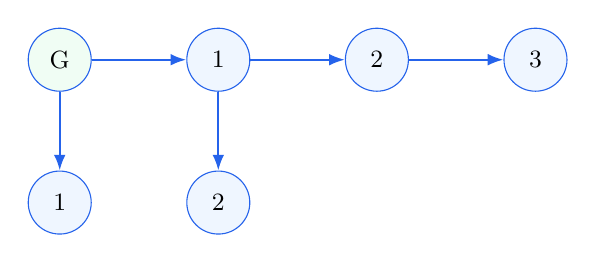
\begin{tikzpicture}[
    node/.style={circle,draw=Accent,fill=SoftBlue,minimum size=8mm,font=\small},
    arrow/.style={-{Latex[length=2mm]},thick,draw=Accent}
]
\node[node,fill=SoftGreen] (g) {G};
\node[node,right=1.2cm of g] (a) {1};
\node[node,below=1.0cm of g] (b) {1};
\node[node,right=1.2cm of a] (c) {2};
\node[node,below=1.0cm of a] (d) {2};
\node[node,right=1.2cm of c] (e) {3};
\draw[arrow] (g) -- (a);
\draw[arrow] (g) -- (b);
\draw[arrow] (a) -- (c);
\draw[arrow] (a) -- (d);
\draw[arrow] (c) -- (e);
\end{tikzpicture}
\end{center}

Trong đề tài, BFS có hai vai trò:

\begin{enumerate}
    \item \term{Tạo nhãn học}: chạy BFS từ goal để tính \code{true\_distance} cho mọi ô reachable.
    \item \term{Làm thuật toán mốc}: dùng BFS để so sánh với A* + Manhattan và A* + ANN.
\end{enumerate}

\begin{warnbox}{Điểm hay bị hỏi}
BFS không dùng để sinh map. Map được sinh ngẫu nhiên trước. Sau đó BFS mới chạy trên map đã có để tính nhãn khoảng cách thật.
\end{warnbox}

\subsection{A* là gì?}

A* là thuật toán tìm kiếm có định hướng. Nó đánh giá mỗi node bằng:

\[
    f(n) = g(n) + h(n)
\]

Trong đó:

\begin{itemize}
    \item \(g(n)\): chi phí đã đi từ start đến node \(n\).
    \item \(h(n)\): chi phí ước lượng từ node \(n\) đến goal.
    \item \(f(n)\): tổng chi phí dự đoán nếu đi qua node \(n\).
\end{itemize}

\begin{teachbox}{Giải thích trực quan}
Nếu BFS giống như tìm kiếm lan đều ra mọi hướng, thì A* giống như người đang cầm bản đồ và ưu tiên đi về phía có vẻ gần đích hơn. Phần ``có vẻ gần đích hơn'' chính là heuristic \(h(n)\).
\end{teachbox}

\subsection{Manhattan heuristic}

Trong lưới 4 hướng, heuristic Manhattan được tính bằng:

\[
    h(n) = |x - x_g| + |y - y_g|
\]

Ví dụ: nếu agent đang ở \((x,y)=(1,17)\), goal ở \((7,7)\), thì:

\[
    h(n) = |1-7| + |17-7| = 6 + 10 = 16
\]

Manhattan rất nhanh nhưng chỉ dùng tọa độ. Nó không học từ dữ liệu và không trực tiếp thấy cấu trúc tường trong mê cung.

\section{Phần Giảng Lý Thuyết 2: ANN Là Gì?}

\subsection{Ý tưởng cơ bản của ANN}

ANN (Artificial Neural Network) là mô hình học máy gồm nhiều lớp tính toán. Nó nhận input, biến đổi qua các lớp ẩn, rồi tạo output. Trong đề tài này, ANN nhận trạng thái mê cung và dự đoán số bước còn lại đến goal.

\begin{center}
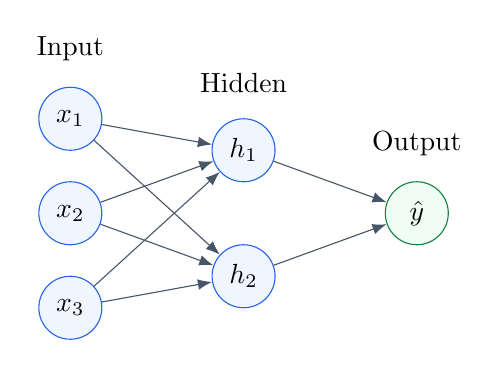
\begin{tikzpicture}[
    neuron/.style={circle,draw=Accent,fill=SoftBlue,minimum size=8mm},
    outputnode/.style={circle,draw=Green,fill=SoftGreen,minimum size=8mm},
    arrow/.style={-{Latex[length=1.8mm]},draw=Muted}
]
\node[neuron] (i1) at (0,1.2) {$x_1$};
\node[neuron] (i2) at (0,0) {$x_2$};
\node[neuron] (i3) at (0,-1.2) {$x_3$};
\node[neuron] (h1) at (2.2,0.8) {$h_1$};
\node[neuron] (h2) at (2.2,-0.8) {$h_2$};
\node[outputnode] (o) at (4.4,0) {$\hat{y}$};
\foreach \i in {i1,i2,i3}{\foreach \h in {h1,h2}{\draw[arrow] (\i) -- (\h);}}
\foreach \h in {h1,h2}{\draw[arrow] (\h) -- (o);}
\node[above=0.2cm of i1] {Input};
\node[above=0.2cm of h1] {Hidden};
\node[above=0.2cm of o] {Output};
\end{tikzpicture}
\end{center}

\subsection{Một neuron tính gì?}

Một neuron nhận nhiều input, nhân với trọng số, cộng bias, rồi đưa qua hàm kích hoạt:

\[
    z = w_1x_1 + w_2x_2 + \cdots + w_nx_n + b = w^Tx + b
\]

\[
    a = \phi(z)
\]

Trong đó \(\phi\) là hàm kích hoạt. Trong đề tài dùng ReLU ở các lớp ẩn:

\[
    \operatorname{ReLU}(z)=\max(0,z)
\]

\begin{teachbox}{Cách giảng dễ hiểu}
Hãy xem mỗi trọng số \(w\) như một núm chỉnh. Nếu một đặc trưng quan trọng, trọng số của nó có thể được học lớn hơn. Nếu đặc trưng ít quan trọng, trọng số có thể nhỏ hơn. Train ANN là quá trình tự động chỉnh các núm này để dự đoán gần nhãn thật hơn.
\end{teachbox}

\subsection{ANN trong đề tài nhận input gì?}

Mỗi trạng thái trong mê cung được đổi thành vector 10 chiều:

\begin{center}
\begin{tabularx}{0.95\linewidth}{>{\bfseries}p{0.27\linewidth}X}
\toprule
Nhóm feature & Ý nghĩa \\
\midrule
\code{x}, \code{y} & Tọa độ hiện tại của agent, đã chuẩn hóa theo kích thước map. \\
\code{goal\_x}, \code{goal\_y} & Tọa độ goal, đã chuẩn hóa. \\
\code{dx}, \code{dy} & Khoảng cách tuyệt đối theo hai trục, gần giống thông tin Manhattan. \\
\code{up\_wall}, \code{down\_wall}, \code{left\_wall}, \code{right\_wall} & Bốn tín hiệu cho biết ô lân cận có phải tường/ngoài biên hay không. \\
\bottomrule
\end{tabularx}
\end{center}

Output của ANN là:

\[
    \hat{y} = \text{dự đoán số bước còn lại đến goal}
\]

Nhãn thật là:

\[
    y = \code{true\_distance} = \text{số bước ngắn nhất do BFS tính}
\]

\begin{teachbox}{Ví dụ một trạng thái cụ thể}
Trong demo đã lưu, start là hàng 17, cột 1; goal là hàng 7, cột 7. Theo code, \(x\) là cột và \(y\) là hàng:

\[
    x=1,\quad y=17,\quad goal_x=7,\quad goal_y=7
\]

Vì map 20x20 nên chia cho 19 để chuẩn hóa:

\[
    x/19 \approx 0.053,\quad y/19 \approx 0.895
\]

Khoảng cách theo trục:

\[
    dx=|1-7|=6,\quad dy=|17-7|=10
\]
\end{teachbox}

\subsection{Kiến trúc ANN dùng trong đề tài}

Mô hình good fit là mô hình chính:

\begin{center}
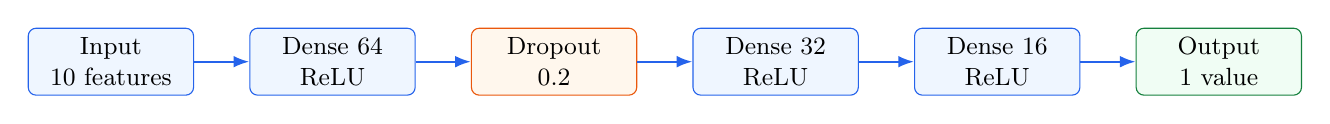
\begin{tikzpicture}[
    block/.style={rectangle,rounded corners=1mm,draw=Accent,fill=SoftBlue,minimum width=2.1cm,minimum height=0.85cm,align=center,font=\small},
    arrow/.style={-{Latex[length=2mm]},thick,draw=Accent}
]
\node[block] (in) {Input\\10 features};
\node[block,right=0.7cm of in] (d1) {Dense 64\\ReLU};
\node[block,right=0.7cm of d1,fill=SoftOrange,draw=Orange] (drop) {Dropout\\0.2};
\node[block,right=0.7cm of drop] (d2) {Dense 32\\ReLU};
\node[block,right=0.7cm of d2] (d3) {Dense 16\\ReLU};
\node[block,right=0.7cm of d3,fill=SoftGreen,draw=Green] (out) {Output\\1 value};
\draw[arrow] (in) -- (d1);
\draw[arrow] (d1) -- (drop);
\draw[arrow] (drop) -- (d2);
\draw[arrow] (d2) -- (d3);
\draw[arrow] (d3) -- (out);
\end{tikzpicture}
\end{center}

\begin{teachbox}{Giải thích Dropout}
Dropout tạm thời bỏ ngẫu nhiên một phần neuron trong lúc train. Mục tiêu là tránh việc mô hình phụ thuộc quá mạnh vào một vài neuron, giúp giảm overfitting.
\end{teachbox}

\section{Phần Giảng Lý Thuyết 3: ANN Học Như Thế Nào?}

\subsection{Forward propagation}

Forward propagation là bước đưa dữ liệu từ input qua mạng để tạo dự đoán.

\begin{center}
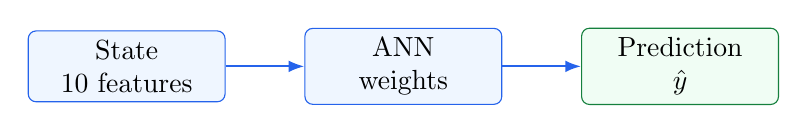
\begin{tikzpicture}[
    block/.style={rectangle,rounded corners=1mm,draw=Accent,fill=SoftBlue,minimum width=2.5cm,minimum height=0.9cm,align=center},
    arrow/.style={-{Latex[length=2mm]},thick,draw=Accent}
]
\node[block] (x) {State\\10 features};
\node[block,right=1cm of x] (net) {ANN\\weights};
\node[block,right=1cm of net,fill=SoftGreen,draw=Green] (pred) {Prediction\\$\hat{y}$};
\draw[arrow] (x) -- (net);
\draw[arrow] (net) -- (pred);
\end{tikzpicture}
\end{center}

Ví dụ: một ô có khoảng cách thật là 20 bước. Model dự đoán 17.5 bước. Khi đó sai số tuyệt đối của mẫu này là 2.5 bước.

\subsection{Loss và metric}

Vì đây là bài toán hồi quy, nhóm dùng MSE làm loss và MAE làm metric.

\[
    \text{MSE}=\frac{1}{n}\sum_{i=1}^{n}(y_i-\hat{y_i})^2
\]

\[
    \text{MAE}=\frac{1}{n}\sum_{i=1}^{n}|y_i-\hat{y_i}|
\]

\begin{teachbox}{Ví dụ tính MAE/MSE bằng tay}
Giả sử có 3 mẫu:
\[
    y=[20,10,15],\quad \hat{y}=[18,13,14]
\]

Sai số tuyệt đối:
\[
    |y-\hat{y}|=[2,3,1]
\]

\[
    MAE=\frac{2+3+1}{3}=2
\]

Sai số bình phương:
\[
    (y-\hat{y})^2=[4,9,1]
\]

\[
    MSE=\frac{4+9+1}{3}=4.67
\]

MAE dễ giải thích vì đơn vị là số bước. MSE phạt lỗi lớn mạnh hơn nên phù hợp làm loss khi train.
\end{teachbox}

\subsection{Backpropagation là gì?}

Sau khi tính loss, mô hình cần biết trọng số nào làm dự đoán sai nhiều. Backpropagation truyền sai số từ output ngược về các lớp trước để tính gradient. Sau đó optimizer Adam cập nhật trọng số.

\begin{center}
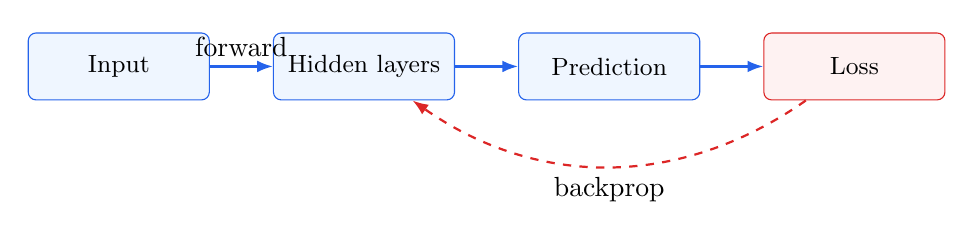
\begin{tikzpicture}[
    block/.style={rectangle,rounded corners=1mm,draw=Accent,fill=SoftBlue,minimum width=2.3cm,minimum height=0.85cm,align=center,font=\small},
    arrow/.style={-{Latex[length=2mm]},thick,draw=Accent},
    back/.style={-{Latex[length=2mm]},thick,dashed,draw=Red}
]
\node[block] (x) {Input};
\node[block,right=0.8cm of x] (h) {Hidden layers};
\node[block,right=0.8cm of h] (p) {Prediction};
\node[block,right=0.8cm of p,fill=SoftRed,draw=Red] (l) {Loss};
\draw[arrow] (x) -- node[above]{forward} (h);
\draw[arrow] (h) -- (p);
\draw[arrow] (p) -- (l);
\draw[back] (l) to[bend left=35] node[below]{backprop} (h);
\end{tikzpicture}
\end{center}

\begin{saybox}{Cách nói dễ hiểu}
Forward là mô hình trả lời: ``tôi đoán còn 17 bước''. Loss cho biết câu trả lời đó sai bao nhiêu so với BFS. Backpropagation là quá trình rút kinh nghiệm: trọng số nào cần tăng, trọng số nào cần giảm để lần sau dự đoán gần đúng hơn.
\end{saybox}

\subsection{Epoch và batch size}

Một epoch là một lần mô hình học qua toàn bộ tập train. Batch size là số mẫu được đưa vào model trong một lần cập nhật. Trong code:

\begin{itemize}
    \item Underfit: 5 epoch, batch size 64.
    \item Overfit: 150 epoch, batch size 32, chỉ dùng 3.000 dòng train.
    \item Good fit: tối đa 100 epoch, batch size 64, EarlyStopping nên dừng ở 20 epoch.
\end{itemize}

\begin{teachbox}{Giải thích epoch bằng ví dụ lớp học}
Nếu tập train giống như một quyển bài tập có 70.000 câu, thì một epoch nghĩa là mô hình đã xem qua toàn bộ 70.000 câu đó một lần. Nếu train 5 epoch, mô hình xem lại quyển bài tập 5 lượt. Xem quá ít có thể chưa hiểu bài; xem quá nhiều với một mô hình quá lớn có thể dẫn đến học vẹt.
\end{teachbox}

\begin{center}
\begin{tikzpicture}[
    block/.style={rectangle,rounded corners=1mm,draw=Accent,fill=SoftBlue,minimum width=2.4cm,minimum height=0.85cm,align=center,font=\small},
    arrow/.style={-{Latex[length=2mm]},thick,draw=Accent}
]
\node[block] (e1) {Epoch 1\\xem hết train};
\node[block,right=0.7cm of e1] (e2) {Epoch 2\\xem lại};
\node[block,right=0.7cm of e2] (e3) {Epoch 3\\cập nhật tiếp};
\node[block,right=0.7cm of e3,fill=SoftGreen,draw=Green] (en) {Epoch n\\loss giảm};
\draw[arrow] (e1) -- (e2);
\draw[arrow] (e2) -- (e3);
\draw[arrow] (e3) -- (en);
\end{tikzpicture}
\end{center}

\section{Phần Quan Trọng: Validation Và Test Khác Nhau Thế Nào?}

\subsection{Ba tập dữ liệu}

Dataset có 100.000 dòng và được chia 70/15/15:

\begin{center}
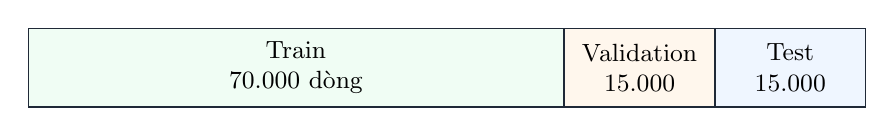
\begin{tikzpicture}[
    part/.style={rectangle,draw=Primary,minimum height=1.0cm,align=center,font=\small},
]
\node[part,fill=SoftGreen,minimum width=6.8cm] (train) at (0,0) {Train\\70.000 dòng};
\node[part,fill=SoftOrange,minimum width=1.9cm,right=0cm of train] (val) {Validation\\15.000};
\node[part,fill=SoftBlue,minimum width=1.9cm,right=0cm of val] (test) {Test\\15.000};
\end{tikzpicture}
\end{center}

\begin{teachbox}{Ví dụ trực quan: học tập, kiểm tra thử, thi cuối kỳ}
Có thể hiểu ba tập dữ liệu giống quá trình học của sinh viên:
\begin{itemize}
    \item \term{Training set}: bài tập để học. Làm sai thì sửa ngay, tương đương model cập nhật trọng số.
    \item \term{Validation set}: bài kiểm tra thử trong lúc ôn. Không dùng để học trực tiếp từng đáp án, nhưng dùng để biết cách học hiện tại có ổn không và có cần đổi cấu hình không.
    \item \term{Testing set}: bài thi cuối kỳ. Chỉ làm một lần sau khi đã học và chọn xong phương pháp. Dùng để báo cáo năng lực cuối cùng.
\end{itemize}
\end{teachbox}

\begin{center}
\begin{tabularx}{0.95\linewidth}{>{\bfseries}p{0.22\linewidth}X}
\toprule
Tập dữ liệu & Dùng để làm gì? \\
\midrule
Train & Cập nhật trọng số của ANN qua backpropagation. Đây là dữ liệu mô hình thật sự học. \\
Validation & Không cập nhật trọng số. Dùng để theo dõi mô hình trong quá trình train, chọn cấu hình, dùng cho EarlyStopping. \\
Test & Không dùng trong lúc chọn mô hình. Chỉ dùng sau cùng để đánh giá kết quả cuối cùng một cách khách quan. \\
\bottomrule
\end{tabularx}
\end{center}

\subsection{Ví dụ trực quan về validation}

Giả sử ta đang thử ba mô hình:

\begin{itemize}
    \item Mô hình A quá nhỏ: validation loss cao.
    \item Mô hình B quá lớn: train loss thấp nhưng validation loss tăng.
    \item Mô hình C vừa phải: validation loss giảm và ổn định.
\end{itemize}

Ta dùng validation để chọn mô hình C. Sau khi đã chọn xong, mới dùng test để báo cáo kết quả cuối cùng.

\subsection{Tại sao cần tách Validation khỏi Test?}

Nếu dùng cùng một tập dữ liệu vừa để chỉnh mô hình vừa để báo cáo điểm cuối cùng, kết quả sẽ không còn khách quan. Khi ta nhìn validation loss để quyết định đổi kiến trúc, thêm Dropout, dùng EarlyStopping hoặc đổi số epoch, ta đang gián tiếp tối ưu theo validation. Vì vậy cần một tập test riêng để ``thi cuối kỳ'' sau khi mọi quyết định đã xong.

\begin{center}
\begin{tabularx}{0.95\linewidth}{>{\bfseries}p{0.27\linewidth}X}
\toprule
Hành động & Dùng tập nào? \\
\midrule
Cập nhật trọng số qua backpropagation & Training set \\
Chọn kiến trúc, theo dõi overfit, EarlyStopping & Validation set \\
Báo cáo kết quả cuối cùng trong bảng metrics & Testing set \\
\bottomrule
\end{tabularx}
\end{center}

\subsection{Quy tắc chia dữ liệu phổ biến}

Không có một tỉ lệ duy nhất đúng cho mọi bài toán, nhưng thường gặp:

\begin{itemize}
    \item \term{70/15/15}: 70\% train, 15\% validation, 15\% test. Đề tài này dùng tỉ lệ này.
    \item \term{80/10/10}: dùng khi muốn dành nhiều dữ liệu hơn cho train.
    \item Nếu dữ liệu rất ít, có thể dùng cross-validation để đánh giá ổn định hơn.
\end{itemize}

\begin{warnbox}{Điểm phản biện hay gặp}
Nếu dùng test nhiều lần để chọn cấu hình, test không còn khách quan. Khi đó mô hình đã ``nhìn gián tiếp'' vào test. Vì vậy trong báo cáo, test chỉ dùng để báo cáo cuối cùng: underfit MAE 2.669, overfit MAE 3.064, good fit MAE 2.284.
\end{warnbox}

\section{Các Chỉ Số Đánh Giá Cần Giải Thích}

\subsection{Accuracy là gì?}

Accuracy là độ chính xác trong bài toán phân loại. Công thức:

\[
    Accuracy = \frac{\text{số mẫu dự đoán đúng}}{\text{tổng số mẫu}}
\]

Ví dụ phân loại ảnh mèo/chó: nếu có 100 ảnh và model đoán đúng 92 ảnh thì Accuracy = 92\%.

\begin{warnbox}{Liên hệ với đề tài}
Đề tài này không dùng Accuracy làm chỉ số chính vì ANN không phân loại ``đúng/sai''. ANN dự đoán một số thực là khoảng cách còn lại đến goal. Vì vậy đây là bài toán hồi quy, dùng MSE và MAE phù hợp hơn.
\end{warnbox}

\subsection{ROC/AUC là gì?}

ROC/AUC thường dùng cho bài toán phân loại nhị phân, ví dụ phân biệt email spam/không spam. Model thường trả về một xác suất. Khi thay đổi ngưỡng quyết định, ta được nhiều cặp:

\begin{itemize}
    \item \term{True Positive Rate}: tỉ lệ mẫu dương được phát hiện đúng.
    \item \term{False Positive Rate}: tỉ lệ mẫu âm bị báo nhầm là dương.
\end{itemize}

ROC curve vẽ True Positive Rate theo False Positive Rate. AUC là diện tích dưới đường ROC. AUC càng gần 1 thì khả năng phân biệt hai lớp càng tốt.

\begin{center}
\begin{tikzpicture}[scale=0.9]
\draw[->] (0,0) -- (5.2,0) node[right]{False Positive Rate};
\draw[->] (0,0) -- (0,4.2) node[above]{True Positive Rate};
\draw[gray,dashed] (0,0) -- (4,4) node[pos=0.65,below right]{ngẫu nhiên};
\draw[Accent,thick] (0,0) .. controls (0.4,2.4) and (1.2,3.4) .. (4,4);
\node[Accent] at (2.9,3.6) {ROC tốt};
\node at (0,-0.3) {0};
\node at (4,-0.3) {1};
\node at (-0.3,4) {1};
\end{tikzpicture}
\end{center}

\begin{warnbox}{Liên hệ với đề tài}
ROC/AUC không phải chỉ số chính của đề tài vì output không phải xác suất phân loại. Tuy nhiên nhóm cần hiểu khái niệm để phân biệt: classification dùng Accuracy/ROC/AUC; regression dùng MSE/MAE.
\end{warnbox}

\subsection{Cross-validation là gì?}

Cross-validation là kỹ thuật kiểm tra chéo dữ liệu. Dữ liệu được chia thành nhiều phần (fold). Mỗi lần chọn một fold làm validation, các fold còn lại làm train. Sau nhiều lần, lấy trung bình kết quả.

\begin{center}
\begin{tikzpicture}[
    fold/.style={rectangle,draw=Primary,minimum height=0.7cm,minimum width=1.6cm,align=center,font=\small}
]
\foreach \i/\x in {1/0,2/1.6,3/3.2,4/4.8,5/6.4}{
    \node[fold,fill=SoftBlue] (f\i) at (\x,0) {Fold \i};
}
\node[fold,fill=SoftOrange] at (0,-1.0) {Val};
\node[fold,fill=SoftGreen] at (1.6,-1.0) {Train};
\node[fold,fill=SoftGreen] at (3.2,-1.0) {Train};
\node[fold,fill=SoftGreen] at (4.8,-1.0) {Train};
\node[fold,fill=SoftGreen] at (6.4,-1.0) {Train};
\node[right] at (8.2,-1.0) {Lần 1};
\node[fold,fill=SoftGreen] at (0,-1.8) {Train};
\node[fold,fill=SoftOrange] at (1.6,-1.8) {Val};
\node[fold,fill=SoftGreen] at (3.2,-1.8) {Train};
\node[fold,fill=SoftGreen] at (4.8,-1.8) {Train};
\node[fold,fill=SoftGreen] at (6.4,-1.8) {Train};
\node[right] at (8.2,-1.8) {Lần 2};
\end{tikzpicture}
\end{center}

Trong đề tài, 5-fold cross-validation của mô hình good fit cho kết quả trung bình:

\[
    \text{Mean MAE}=2.223,\qquad \text{Mean MSE}=14.859
\]

Ý nghĩa: kết quả không chỉ tốt ở một lần chia dữ liệu duy nhất, mà tương đối ổn định qua nhiều cách chia.

\subsection{Đọc đồ thị Loss/Accuracy qua các Epoch}

Với bài toán phân loại, ta thường nhìn loss và accuracy theo epoch. Với bài toán hồi quy như đề tài này, ta nhìn loss và MAE theo epoch. Cách đọc vẫn giống nhau: so sánh đường train và validation.

\begin{center}
\begin{tikzpicture}[scale=0.9]
\draw[->] (0,0) -- (5.2,0) node[right]{Epoch};
\draw[->] (0,0) -- (0,3.6) node[above]{Loss};
\draw[Green,thick] (0.3,3.0) .. controls (1.5,1.7) and (3.0,1.1) .. (4.8,0.8);
\draw[Orange,thick] (0.3,3.1) .. controls (1.5,1.8) and (3.0,1.2) .. (4.8,1.0);
\node[Green] at (4.5,0.55) {train};
\node[Orange] at (4.5,1.3) {validation};
\node at (2.5,-0.55) {Good fit: cả hai cùng giảm rồi ổn định};
\end{tikzpicture}
\end{center}

\begin{center}
\begin{tabularx}{0.95\linewidth}{>{\bfseries}p{0.28\linewidth}X}
\toprule
Dạng đồ thị & Cách hiểu \\
\midrule
Train loss và validation loss đều cao & Underfitting: mô hình chưa học đủ. \\
Train loss giảm, validation loss tăng/xấu & Overfitting: mô hình học quá kỹ train. \\
Train loss và validation loss cùng giảm rồi ổn định & Good fit: mô hình học tương đối tốt và tổng quát hơn. \\
\bottomrule
\end{tabularx}
\end{center}

\begin{saybox}{Câu nói khi trình bày phần chỉ số}
Trong bài này, em vẫn giải thích Accuracy và ROC/AUC vì đây là các chỉ số học máy phổ biến. Tuy nhiên vì mô hình của nhóm dự đoán số bước còn lại, không phân loại nhãn, nên chỉ số chính của đề tài là MSE và MAE. Đồ thị nhóm xuất ra là loss và MAE theo epoch, tương đương cách đọc loss/accuracy trong bài toán phân loại.
\end{saybox}

\section{Dữ Liệu Được Tạo Như Thế Nào?}

\subsection{Pipeline tạo dataset}

\begin{center}
\begin{tikzpicture}[
    block/.style={rectangle,rounded corners=1mm,draw=Accent,fill=SoftBlue,minimum width=2.8cm,minimum height=1.0cm,align=center,font=\small},
    arrow/.style={-{Latex[length=2mm]},thick,draw=Accent}
]
\node[block] (map) {Sinh map\\ngẫu nhiên};
\node[block,right=0.7cm of map] (goal) {Chọn goal\\hợp lệ};
\node[block,right=0.7cm of goal] (bfs) {BFS từ goal\\tính khoảng cách};
\node[block,right=0.7cm of bfs] (feat) {Trích xuất\\10 feature};
\node[block,right=0.7cm of feat] (csv) {CSV\\100.000 dòng};
\draw[arrow] (map) -- (goal);
\draw[arrow] (goal) -- (bfs);
\draw[arrow] (bfs) -- (feat);
\draw[arrow] (feat) -- (csv);
\end{tikzpicture}
\end{center}

\begin{teachbox}{Liên hệ code}
\begin{itemize}
    \item \code{dataset.py}: sinh từng map, chọn goal, chạy \code{bfs\_distances\_to\_goal}.
    \item \code{features.py}: đổi mỗi ô reachable thành vector 10 feature.
    \item \code{generate\_dataset.py}: tạo file \code{data/maze\_dataset.csv}.
\end{itemize}
\end{teachbox}

\subsection{Vì sao chạy BFS từ goal?}

Nếu chạy BFS riêng cho từng ô, mỗi ô phải chạy một lần, rất tốn thời gian. Thay vào đó, chạy BFS một lần từ goal sẽ thu được khoảng cách ngắn nhất từ mọi ô reachable đến goal.

\begin{saybox}{Cách nói trên lớp}
Ta có thể xem goal như trung tâm phát sóng. BFS lan từ goal ra ngoài; ô nào được chạm ở lớp thứ 5 thì cách goal 5 bước, ô nào ở lớp thứ 20 thì cách goal 20 bước. Như vậy một lần BFS tạo được nhãn cho nhiều trạng thái.
\end{saybox}

\section{Ba Trạng Thái Thực Nghiệm Của Mô Hình}

\subsection{Underfitting}

Underfitting xảy ra khi mô hình quá đơn giản hoặc học quá ít, nên không bắt được quy luật dữ liệu.

\begin{figure}[H]
    \centering
    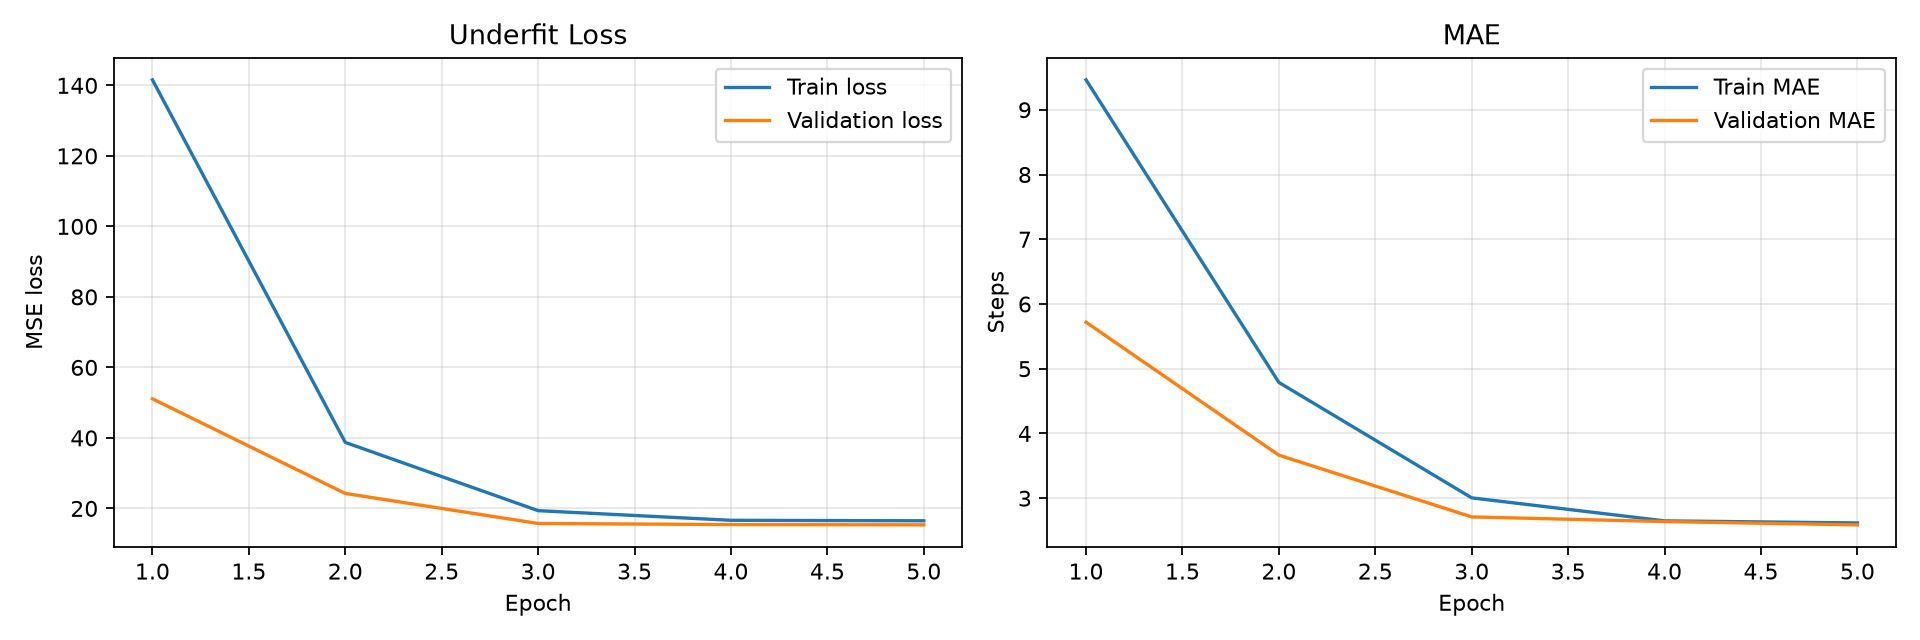
\includegraphics[width=0.88\linewidth]{underfit_loss.png}
    \caption{Đồ thị huấn luyện thật của mô hình underfit}
\end{figure}

\begin{saybox}{Cách trình bày hình underfit}
Ở thí nghiệm underfit, mạng chỉ có Dense(4) và output, train 5 epoch. Mô hình quá nhỏ nên sai số test còn cao: Test MSE = 16.322, Test MAE = 2.669. Khi nói, chỉ vào đồ thị loss và MAE để nhấn mạnh rằng mô hình chưa học đủ tốt.
\end{saybox}

\subsection{Overfitting}

Overfitting xảy ra khi mô hình học quá kỹ tập train nhưng tổng quát kém trên validation/test. Trong đề tài, overfit được tạo bằng mạng lớn và chỉ train trên 3.000 dòng.

\begin{figure}[H]
    \centering
    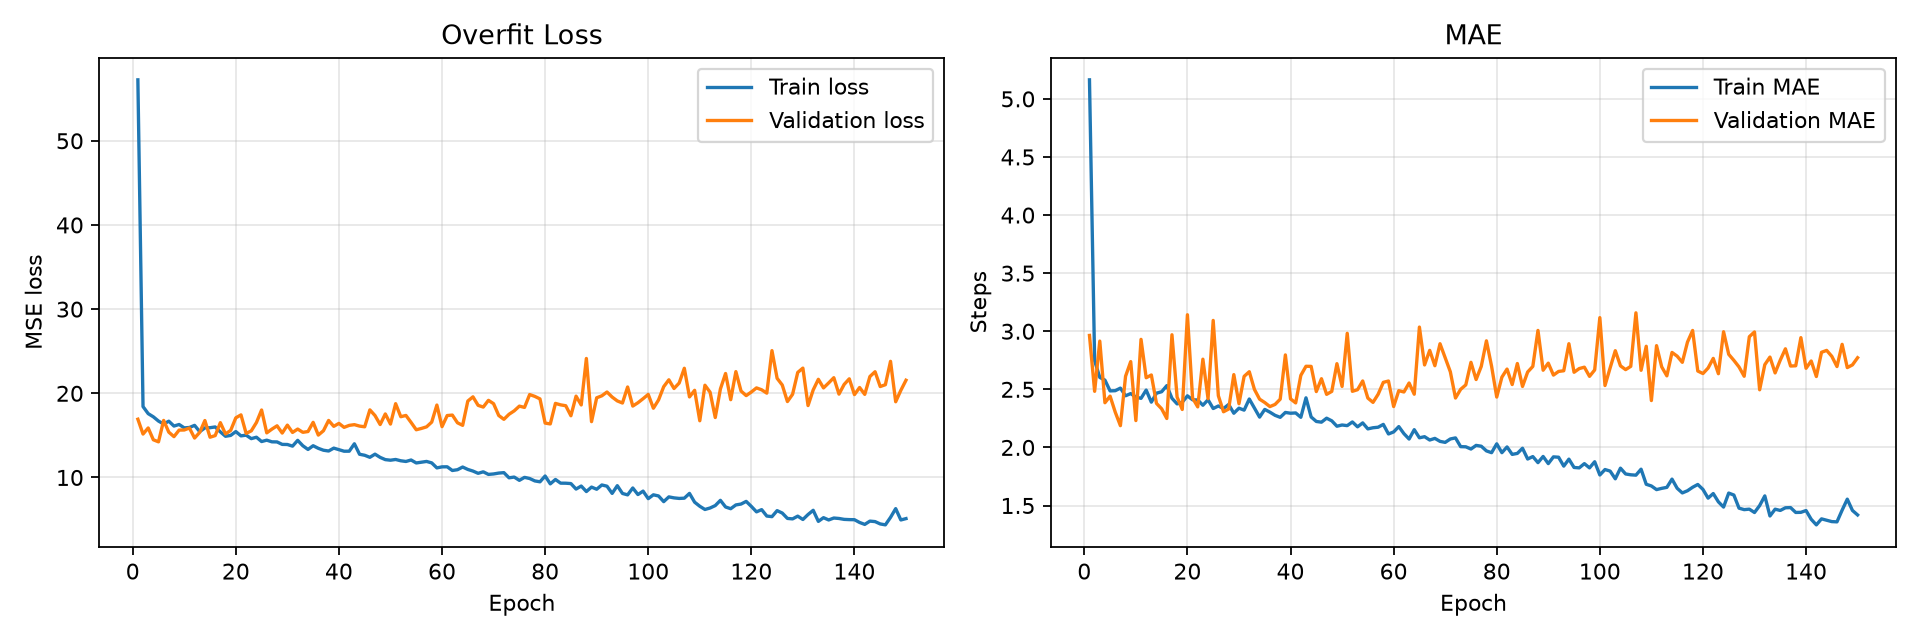
\includegraphics[width=0.88\linewidth]{overfit_loss.png}
    \caption{Đồ thị huấn luyện thật của mô hình overfit}
\end{figure}

\begin{saybox}{Cách trình bày hình overfit}
Mạng overfit có Dense(512), Dense(512), Dense(256), Dense(128), train 150 epoch nhưng chỉ dùng 3.000 dòng train. Dấu hiệu cần chỉ ra là train loss có thể giảm nhưng validation loss không tốt tương ứng. Test MAE = 3.064, kém hơn good fit.
\end{saybox}

\subsection{Good fit}

Good fit là trạng thái mô hình học đủ tốt trên train và vẫn tổng quát tốt trên validation/test. Mô hình chính dùng Dense(64), Dropout(0.2), Dense(32), Dense(16), output.

\begin{figure}[H]
    \centering
    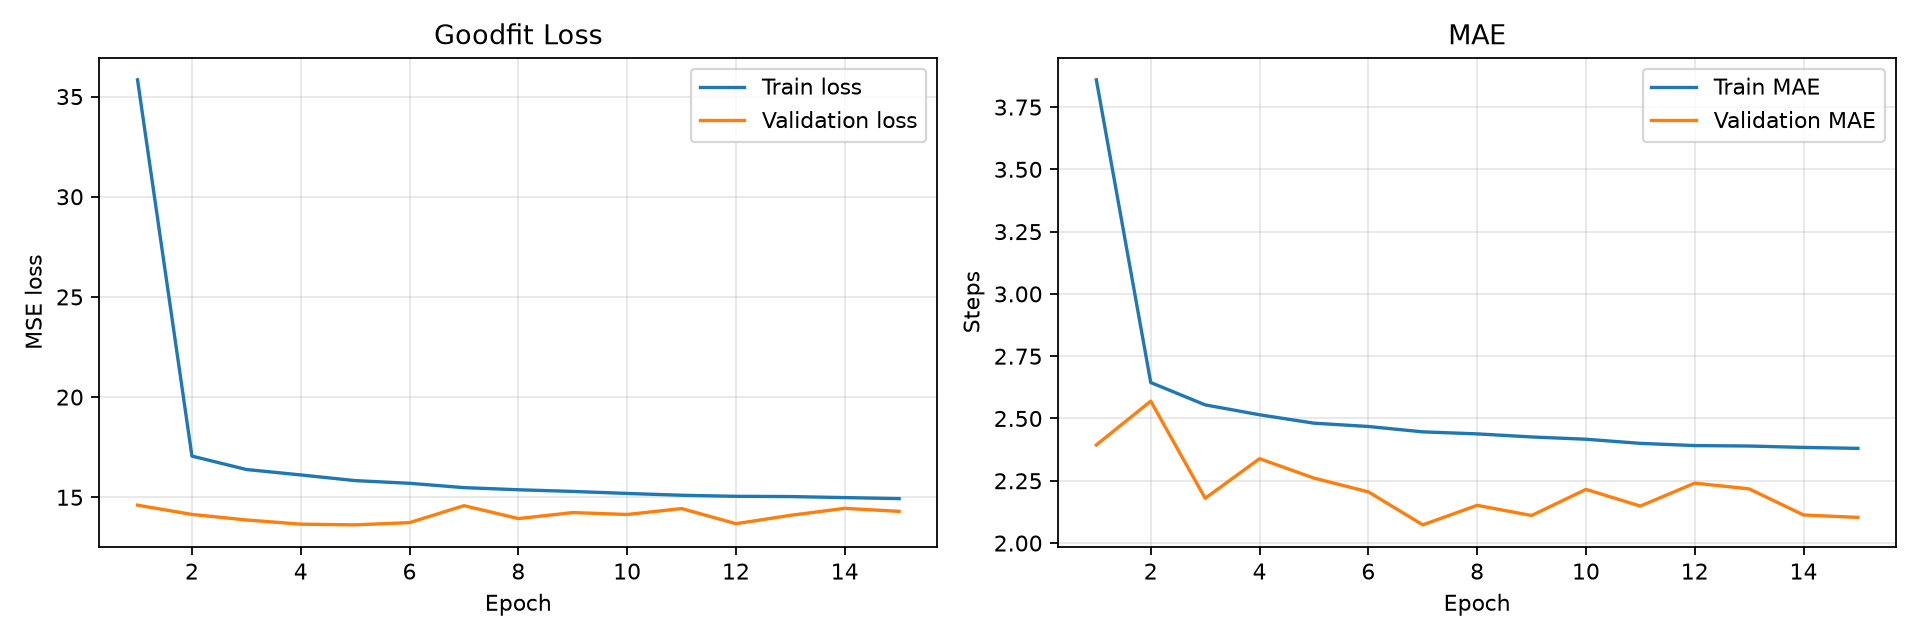
\includegraphics[width=0.88\linewidth]{goodfit_loss.png}
    \caption{Đồ thị huấn luyện thật của mô hình good fit}
\end{figure}

\begin{saybox}{Cách trình bày hình good fit}
Mô hình good fit có kiến trúc vừa phải, dùng Dropout và EarlyStopping. Cấu hình tối đa 100 epoch nhưng dừng ở 20 epoch vì validation loss không cải thiện thêm. Kết quả tốt nhất: Test MSE = 14.300, Test MAE = 2.284.
\end{saybox}

\subsection{Bảng so sánh ba thí nghiệm}

\begin{center}
\begin{tabular}{lrrrr}
\toprule
Mô hình & Train rows & Epoch & Test MSE & Test MAE \\
\midrule
Underfit & 70.000 & 5 & 16.322 & 2.669 \\
Overfit & 3.000 & 150 & 24.811 & 3.064 \\
Good fit & 70.000 & 20 & 14.300 & 2.284 \\
\bottomrule
\end{tabular}
\end{center}

\section{Tích Hợp ANN Vào A*}

\subsection{Từ model thành heuristic}

Sau khi train, model good fit được lưu thành:

\begin{itemize}
    \item \code{models/ann\_heuristic\_goodfit.keras}: model Keras.
    \item \code{models/ann\_heuristic\_goodfit.tflite}: bản TensorFlow Lite để suy luận trong demo.
\end{itemize}

Trong A*, chỉ cần một hàm heuristic có dạng:

\begin{lstlisting}
heuristic(position, goal) -> float
\end{lstlisting}

\code{AnnHeuristic} trong \code{heuristics.py} làm đúng việc này: nhận \code{position}, \code{goal}, gọi \code{state\_to\_features}, đưa vào TFLite model và trả về dự đoán khoảng cách.

\begin{center}
\begin{tikzpicture}[
    block/.style={rectangle,rounded corners=1mm,draw=Accent,fill=SoftBlue,minimum width=2.8cm,minimum height=1.0cm,align=center,font=\small},
    arrow/.style={-{Latex[length=2mm]},thick,draw=Accent}
]
\node[block] (state) {Node hiện tại\\trong A*};
\node[block,right=0.8cm of state] (features) {10 features};
\node[block,right=0.8cm of features] (ann) {ANN model};
\node[block,right=0.8cm of ann,fill=SoftGreen,draw=Green] (h) {$h_{ANN}(n)$};
\node[block,below=1.1cm of h,fill=SoftOrange,draw=Orange] (astar) {$f(n)=g(n)+h(n)$};
\draw[arrow] (state) -- (features);
\draw[arrow] (features) -- (ann);
\draw[arrow] (ann) -- (h);
\draw[arrow] (h) -- (astar);
\end{tikzpicture}
\end{center}

\subsection{Demo kết quả}

\begin{figure}[H]
    \centering
    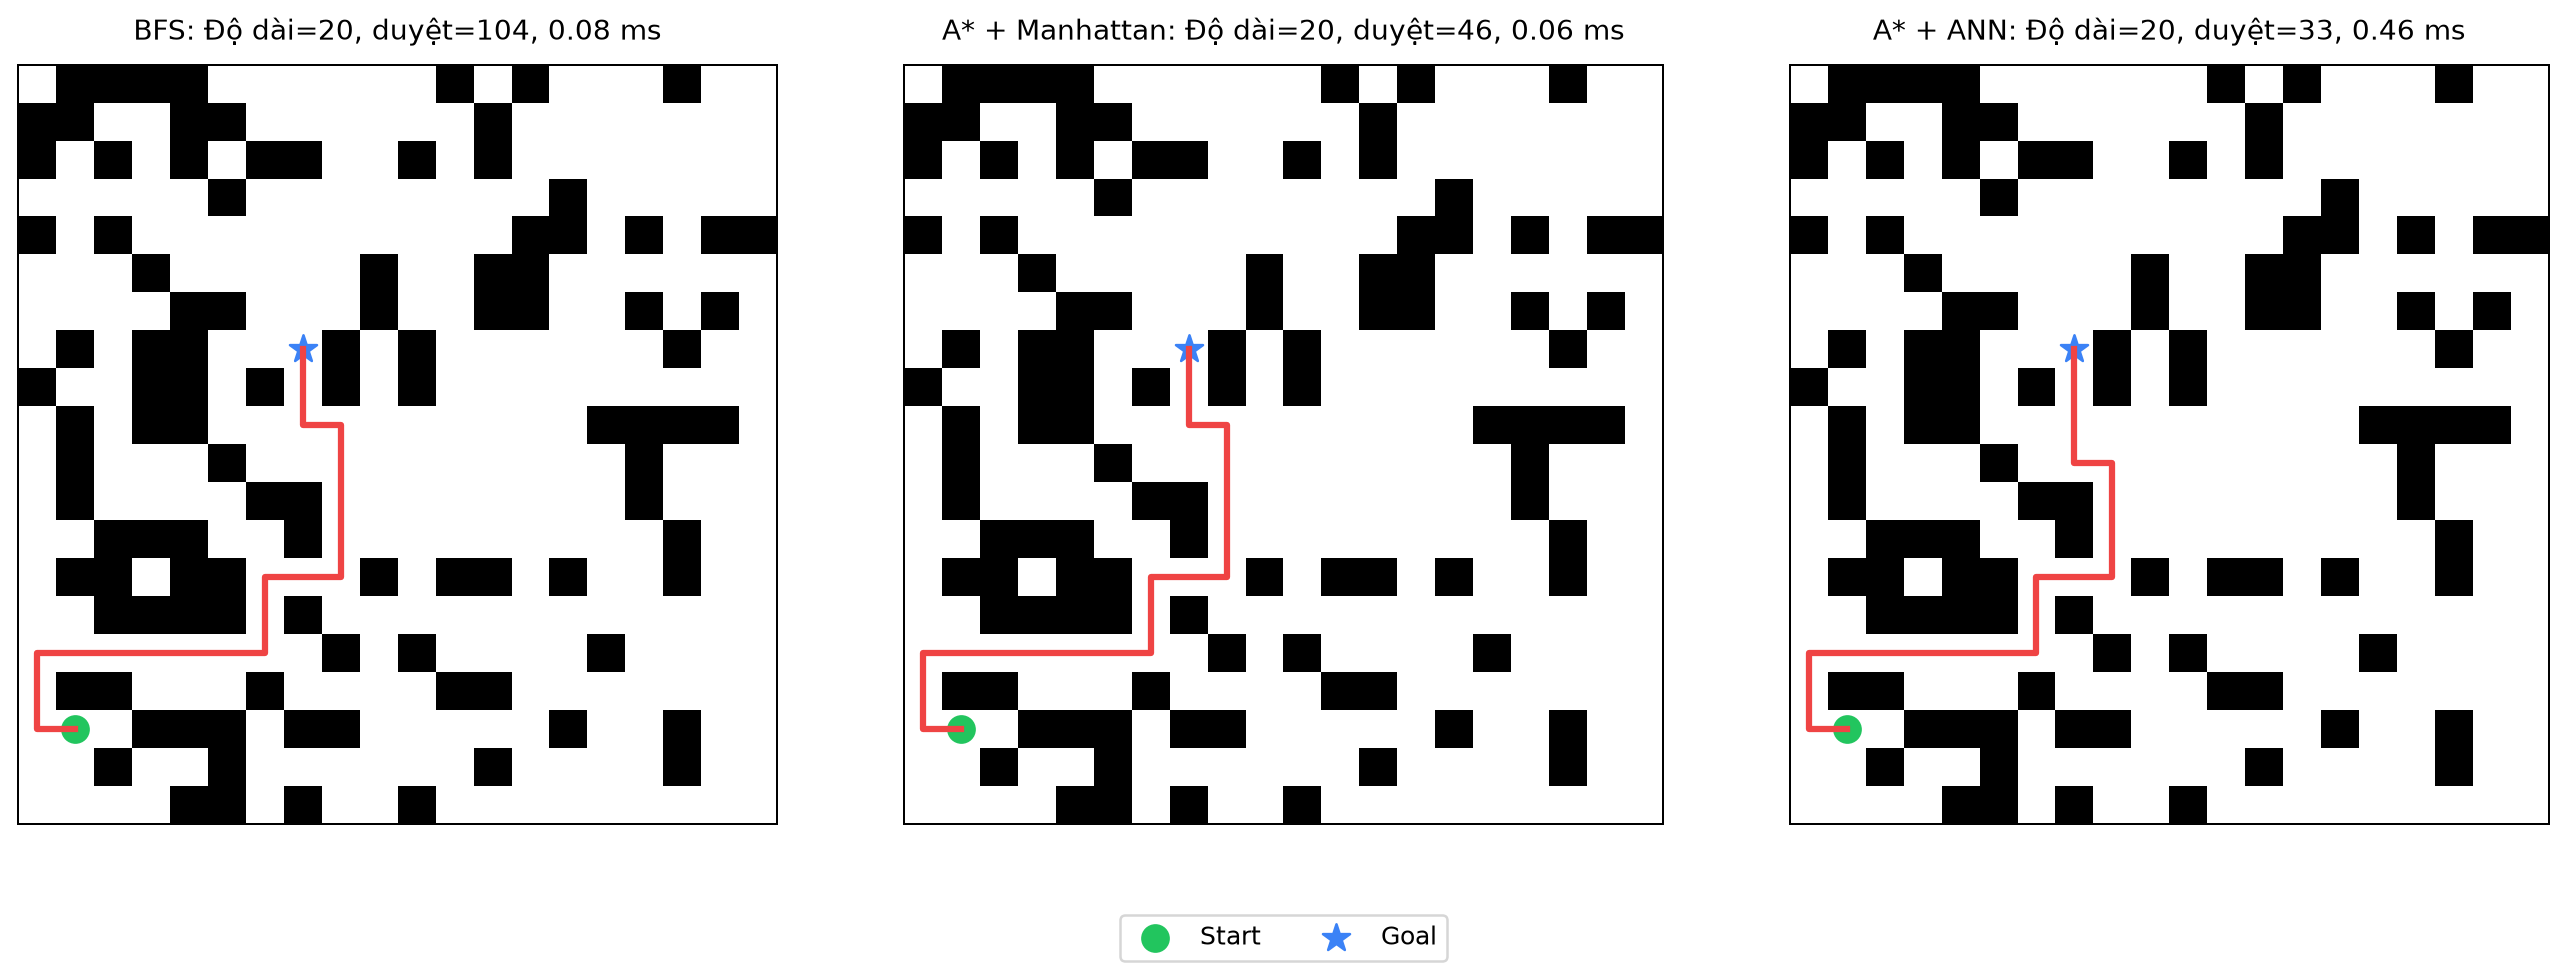
\includegraphics[width=0.82\linewidth]{demo_path.png}
    \caption{Ảnh demo so sánh BFS, A* + Manhattan và A* + ANN}
\end{figure}

\begin{center}
\begin{tabular}{lrrr}
\toprule
Thuật toán & Độ dài path & Node duyệt & Thời gian \\
\midrule
BFS & 20 & 104 & 0.09 ms \\
A* + Manhattan & 20 & 46 & 0.07 ms \\
A* + ANN & 20 & 33 & 0.48 ms \\
\bottomrule
\end{tabular}
\end{center}

\begin{saybox}{Cách nói khi demo}
Trong demo này, cả ba thuật toán đều tìm được đường dài 20 bước. BFS duyệt nhiều nhất vì không có heuristic. A* + Manhattan giảm node duyệt nhờ định hướng theo tọa độ. A* + ANN duyệt 33 node, ít nhất trong demo, vì heuristic học từ dữ liệu tạo thứ tự ưu tiên khác Manhattan. Tuy nhiên thời gian ANN cao hơn Manhattan do phải gọi model suy luận.
\end{saybox}

\section{Kịch Bản Thuyết Trình Theo Slide}

\subsection*{Slide 1: Tên đề tài}
\begin{saybox}{Nói}
Nhóm em trình bày đề tài ứng dụng ANN làm heuristic cho A*. Thay vì chỉ dùng công thức Manhattan cố định, nhóm em huấn luyện một model để dự đoán chi phí còn lại đến goal.
\end{saybox}

\subsection*{Slide 2: Mục tiêu}
\begin{saybox}{Nói}
Mục tiêu gồm ba phần: hiểu ANN học như thế nào, chứng minh ba trạng thái underfit-overfit-goodfit bằng đồ thị train thật, và tích hợp ANN vào A* để demo so sánh.
\end{saybox}

\subsection*{Slide 3--6: BFS, A*, Manhattan}
\begin{saybox}{Nói}
Trước khi vào ANN, em giải thích thuật toán nền. BFS đảm bảo khoảng cách ngắn nhất trong lưới không trọng số nhưng duyệt nhiều. A* dùng \(f(n)=g(n)+h(n)\). Manhattan là heuristic đơn giản dựa trên tọa độ, nhanh nhưng không học từ dữ liệu.
\end{saybox}

\subsection*{Slide 7--11: ANN và dữ liệu}
\begin{saybox}{Nói}
ANN nhận 10 feature của trạng thái, gồm tọa độ, khoảng cách tương đối và tường lân cận. Output là khoảng cách còn lại. Nhãn khoảng cách được BFS tính. Đây là bài toán hồi quy nên dùng MSE/MAE, không dùng Accuracy.
\end{saybox}

\subsection*{Slide 12--14: Underfit, overfit, good fit}
\begin{saybox}{Nói}
Ba slide này là phần thực nghiệm quan trọng nhất. Em sẽ chỉ vào từng đồ thị: underfit do mạng quá nhỏ, overfit do mạng quá lớn và train lâu trên ít dữ liệu, good fit do cấu hình vừa phải có Dropout và EarlyStopping. Mô hình good fit là mô hình dùng cho demo A* + ANN.
\end{saybox}

\subsection*{Slide 15--16: Cross-validation và demo}
\begin{saybox}{Nói}
Cross-validation kiểm tra kết quả có ổn định không. Demo cho thấy khi tích hợp ANN vào A*, số node duyệt trong map minh họa giảm còn 33, thấp hơn BFS và A* + Manhattan.
\end{saybox}

\subsection*{Slide 17--18: Nhận xét, hạn chế, minh bạch AI}
\begin{saybox}{Nói}
Nhóm không khẳng định ANN luôn thắng Manhattan. Kết quả chứng minh pipeline hoạt động và có demo minh họa. AI hỗ trợ khung code/debug/tổ chức nội dung; nhóm tự chạy lại kết quả, train model và giải thích số liệu.
\end{saybox}

\section{Kịch Bản Demo Trực Tiếp}

\subsection{Lệnh chạy}

\begin{lstlisting}
python -m src.ui
\end{lstlisting}

\subsection{Thao tác}

\begin{enumerate}
    \item Nhấn \code{R} để random map mới.
    \item Nhấn \code{A} hoặc \code{Run All} để chạy BFS, A* + Manhattan, A* + ANN.
    \item Cho người xem thấy node được animate và đánh số.
    \item Nhấn \code{0} hoặc \code{Show All} để hiển thị cả ba path.
    \item Nếu cần chạy riêng: \code{1} là BFS, \code{2} là A* + Manhattan, \code{3} là A* + ANN.
\end{enumerate}

\begin{warnbox}{Nếu demo live lỗi}
Nếu máy không mở được Pygame hoặc TensorFlow, dùng ảnh tĩnh \code{outputs/demo\_path.png} và bảng \code{outputs/demo\_metrics.json}. Nói rõ đây là kết quả đã chạy trước từ cùng mã nguồn.
\end{warnbox}

\section{Giải Thích Mã Nguồn Theo Module}

\begin{small}
\begin{longtable}{>{\bfseries\raggedright\arraybackslash}p{0.28\linewidth}p{0.62\linewidth}}
\toprule
File & Vai trò cần nắm \\
\midrule
\code{maze.py} & Sinh map ngẫu nhiên, định nghĩa ô tường/đường đi, duyệt 4 láng giềng. \\
\code{dataset.py} & Sinh nhiều map, chọn goal, chạy BFS để lấy khoảng cách thật. \\
\code{features.py} & Tạo 10 feature, tạo dòng dataset, tách \code{X} và \code{y}. \\
\code{search.py} & Cài BFS, A*, Manhattan, reconstruct path, lưu thứ tự node duyệt. \\
\code{models.py} & Định nghĩa underfit, overfit, good fit bằng \code{tf.keras}. \\
\code{train.py} & Chia train/validation/test, train model, lưu \code{.keras}, export \code{.tflite}, vẽ loss. \\
\code{cross\_validate.py} & Chạy 5-fold cross-validation. \\
\code{heuristics.py} & Bọc TFLite model thành hàm heuristic cho A*. \\
\code{demo.py} & Chạy so sánh và lưu ảnh/metrics. \\
\code{ui.py} & UI Pygame: random map, run all, animate node, show path. \\
\bottomrule
\end{longtable}
\end{small}

\section{Câu Hỏi Phản Biện Và Trả Lời}

\begin{teachbox}{1. ANN trong bài này là gì?}
ANN là mô hình hồi quy nhận 10 feature của trạng thái mê cung và dự đoán khoảng cách còn lại đến goal. Model được xây bằng Keras qua \code{tf.keras.Sequential}.
\end{teachbox}

\begin{teachbox}{2. Model học như thế nào?}
Forward tạo dự đoán, MSE đo sai số, backpropagation tính gradient, Adam cập nhật trọng số. Quá trình lặp qua nhiều epoch.
\end{teachbox}

\begin{teachbox}{3. Validation và Test khác nhau thế nào?}
Validation dùng trong quá trình chọn cấu hình và EarlyStopping; test chỉ dùng cuối cùng để đánh giá khách quan. Không dùng test để điều chỉnh model.
\end{teachbox}

\begin{teachbox}{4. Có dùng Keras không?}
Có. Code dùng \code{tf.keras.Sequential}, \code{Dense}, \code{Dropout}, \code{Adam}, \code{MeanAbsoluteError}, \code{EarlyStopping}. File model lưu ở định dạng \code{.keras}.
\end{teachbox}

\begin{teachbox}{5. BFS có sinh map không?}
Không. Map sinh ngẫu nhiên. BFS dùng để gán nhãn \code{true\_distance} và làm thuật toán mốc so sánh.
\end{teachbox}

\begin{teachbox}{6. Vì sao A* + ANN chậm hơn Manhattan nhưng vẫn được dùng?}
Manhattan là công thức rất nhanh. ANN phải gọi model suy luận nên chậm hơn, nhưng mục tiêu đề tài là chứng minh có thể tích hợp heuristic học từ dữ liệu vào A* và so sánh số node duyệt.
\end{teachbox}

\section{Kết Bài}

\begin{saybox}{Câu kết nên học thuộc}
Qua đề tài này, nhóm em xây dựng được một pipeline hoàn chỉnh: sinh map ngẫu nhiên, dùng BFS tạo nhãn, train ANN bằng Keras, phân tích underfit-overfit-goodfit bằng đồ thị train thật, và tích hợp mô hình good fit vào A*. Điểm chính của đề tài là sự kết hợp giữa thuật toán tìm kiếm truyền thống và heuristic học từ dữ liệu.
\end{saybox}

\end{document}
